\\*************************************************************************\\

\documentclass[10pt,a4paper]{article}

\usepackage[utf8]{inputenc}
\usepackage[margin=1in]{geometry}
\thispagestyle{empty}

\usepackage[spanish]{babel}

\usepackage{amsmath}
\usepackage{amsfonts}
\usepackage{amssymb}

\usepackage{parskip}

\usepackage{listings}
\usepackage{xcolor}

\usepackage{enumerate}

\usepackage{hyperref}

\usepackage{float}
\restylefloat{figure}
\usepackage[font=small,labelfont=bf]{caption}
\usepackage{wrapfig}

\usepackage{graphicx}
\restylefloat{figure}

\usepackage{cancel}

\usepackage{multicol}
\setlength{\columnsep}{22pt}

\usepackage{colortbl}

\usepackage{cases}

\usepackage{verbatim}

\title{Título}
\author{Cristian Escudero \\ \small{Subtítulo}}

\begin{document}
\maketitle

\\*************************************************************************\\

\begin{figure}[ht!]
  \caption{Cuerpo siendo deformado.}
  \label{fig:fig1}
  \centering
  \hbox{\includegraphics[width=\textwidth-\fboxrule-\fboxrule]{plot_1.png}}
\end{figure}

\begin{wrapfigure}{r}{0.5\textwidth}
  \caption{Cuerpo siendo deformado.}
  \label{fig:fig1}
  \centering
  \hbox{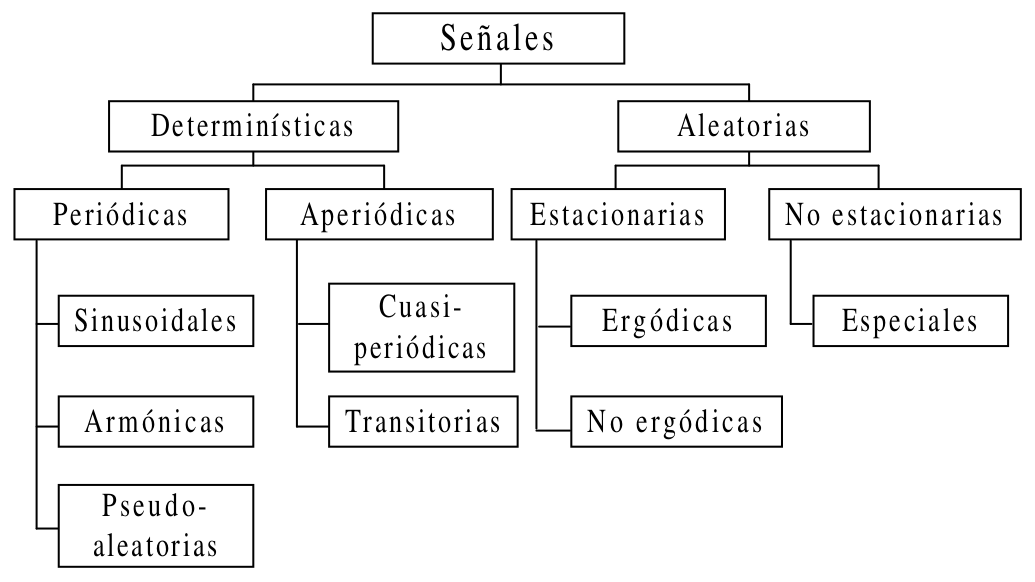
\includegraphics[width=0.5\textwidth-\fboxrule-\fboxrule]{fig1.png}}
\end{wrapfigure}

\lstset { 
  language=Octave,
  basicstyle=\footnotesize,
  numbers=left,
  numberstyle=\tiny\color{cyan},
  stepnumber=1,
  numbersep=8pt,
  backgroundcolor=\color{white},
  showspaces=false,               % show spaces adding particular underscores
  showstringspaces=false,         % underline spaces within strings
  frame=lines,                   % adds a frame around the code
  rulecolor=\color{cyan},
  tabsize=4,                      
  captionpos=b,                   % sets the caption-position to bottom
  breaklines=true,                % sets automatic line breaking
  keywordstyle=\color{blue},          % keyword style
  commentstyle=\color{gray},       % comment style
  stringstyle=\color{magenta},         % string literal style
}

\begin{lstlisting}
\end{lstlisting}

\begin{table}[h]
\centering
\begin{tabular}{ | c | c | c | c | c | c | c | }
\hline
$i$ & $x_i$ & $f(x_i)$ & $a_i$ & $b_i$ & $c_i$ & $d_i$ \\
  \hline
0	&0.9	&1.3	&1.3	&0.0000	&2.2813	&-2.5783\\
1	&1.3	&1.5	&1.5	&0.5875	&-0.8126	&1.3428\\
2	&1.9	&1.85	&1.85	&1.0626	&1.6045	&-3.3374\\
3	&2.1	&2.1	&2.1	&1.3039	&-0.398	&-0.4196\\
4	&2.6	&2.6	&2.6	&0.5912	&-1.0274	&0.4362\\
5	&3.0	&2.7	&2.7	&-0.0214	&-0.504	&0.1749\\	
6	&3.9	&2.4	&2.4	&-0.5036	&-0.0317	&0.0776\\
7	&4.4	&2.15	&2.15	&-0.477	&0.0847	&1.3144\\
8	&4.7	&2.05	&2.05	&-0.0713	&1.2677	&-1.5813\\
9	&5.0	&2.1	&2.1	&0.2623	&-0.1555	&0.0431\\
10	&6.0	&2.25	&2.25	&0.0808	&-0.0261	&-0.0047\\
11	&7.0	&2.3	&2.3	&0.0146	&-0.0401	&-0.0244\\
12	&8.0	&2.25	&2.25	&-0.139	&-0.1134	&0.0174\\
13	&9.2	&1.95	&1.95	&-0.3359	&-0.0507	&-0.0126\\
14	&10.5	&1.4	&1.4	&-0.5315	&-0.0997	&-0.0214\\
15	&11.3	&0.9	&0.9	&-0.7322	&-0.1512	&1.2324\\
16	&11.6	&0.7	&0.7	&-0.4902	&0.958	&-0.8937\\
17	&12.0	&0.6	&0.6	&-0.1528	&-0.1145	&0.1522\\
18	&12.6	&0.5	&0.5	&-0.1257	&0.1595	&-1.1755\\
19	&13.0	&0.4	&0.4	&-0.5623	&-1.2511	&4.8629\\
20	&13.3	&0.25	&0.25	&0.0000	&3.1255	&0.0000\\
\hline
\end{tabular}
\caption{Resultados obtenidos del inciso (a).}
\label{tab:myfirsttable}
\end{table}

\begin{tabular}{rl}
{\bf First Column} & {\bf Second Column} \\\hline \\ [-1.5ex]
First Item & First Attribute \\
& Second Attribute \\
& Third Attribute \\ [1ex] \hline \\ [-1.5ex]
Second Item & First Attribute \\
& Second Attribute \\
& Third Attribute \\
& Fourth Attribute \\ [1ex] \hline \\ [-1.5ex]
Third Item & First Attribute \\
& Second Attribute \\ [1ex] \hline \\ [-1.5ex]
Fourth Item & First Attribute \\
& Second Attribute \\
& Third Attribute \\ [1ex] \hline \\ [-1.5ex]
\end{tabular}
